
\begin{figure}
    \centering
    \includegraphics[width=0.92\textwidth]{images/mass_effect3_smoke.jpg}
    \caption{Animação de fumaça no jogo \textit{Mass Effect 3}.}
    \subcaption*{Fonte: \url{https://www.fxguide.com/fxfeatured/cinematics-case-study-mass-effect-3/}}
    \label{fig:masseffect3}
\end{figure}

As indústrias do entretenimento, jogos (\figref{fig:masseffect3}) e engenharia têm grande interesse em simulações de fluidos para integrar em seus respectivos produtos. Em geral, simulações baseadas em física tendem a apresentar resultados visualmente realísticos e convincentes, podendo levar uma pessoa leiga na área a confundir uma gravação real com uma simulação \cite{Huang2015}. É necessário que o observador da simulação seja convencido de sua veracidade, pois isso aumenta a imersão na experiência de um filme ou jogo. Para alcançar esse nível de qualidade desejado, é preciso trabalhar com técnicas computacionalmente custosas para minimizar a perda de detalhes na simulação. Portanto, é importante utilizar métodos com alta precisão e otimização do tempo de execução para poder aplicar a técnica em tempo real, no caso de jogos, e poupar tempo na produção de efeitos especiais em filmes.

O comportamento de fluidos no mundo real é descrito de maneira contínua. Quando se discretiza este fenômeno para simular computacionalmente, é necessário realizar um passo de discretização do domínio. Por conta disto, simulações de fluidos podem ser abordadas de duas maneiras mais comumente usadas: visão lagrangiana e visão euleriana, além da forma híbrida.

Na visão lagrangiana (ver \figref{fig:lagrangiana}), o fluido é discretizado em forma de um sistema de partículas, com cada uma delas representando uma parte da massa fluídica (volume). Cada partícula tem uma posição no domínio e carrega consigo algumas propriedades daquela parte do fluido que a mesma está discretizando, como velocidade, posição, pressão e força externa. A simulação é realizada pela determinação, em cada passo de tempo, da posição e velocidade de cada partícula do sistema. Já na abordagem euleriana (ver \figref{fig:euleriana}), a discretização do espaço é feita em uma grade ou malha. Esta grade é dividida em células, e estas armazenam as propriedades do fluido que estão passando por aquela região do espaço, sendo responsáveis por gerir como o fluido irá escoar.

\begin{figure}
    \centering
    \caption{Tipos de simulações de escoamento de fluidos}
    \begin{subfigure}[b]{0.45\textwidth}
        \centering
        \includegraphics[width=\textwidth]{images/lagrangeana.pdf}
        \caption{Simulação pela visão lagrangiana.}
        \label{fig:lagrangiana}
    \end{subfigure}
    \hfill
    \begin{subfigure}[b]{0.45\textwidth}
        \centering
        \includegraphics[width=\textwidth]{images/euleriana.pdf}
        \caption{Simulação pela visão euleriana.}
        \label{fig:euleriana}
    \end{subfigure}
    \subcaption*{Fonte: Elaborada pelo autor.}
    \label{fig:simulacoes}
\end{figure}

Existem diversas características que diferem na representação da malha. Por exemplo, existem malhas regulares e irregulares. Em malhas regulares, os centros de cada célula são equidistantes e colineares, enquanto nas malhas irregulares não existe esta restrição. Outro fator que pode distinguir é a topologia de cada célula da malha: existem malhas com topologia triangular, quadrangular ou mistas. Malhas triangulares se moldam melhor em fronteiras irregulares, como objetos complexos, porém, este benefício é contrabalançado pelo grande custo computacional. Malhas quadrangulares têm a desvantagem de perder muitos detalhes por conta da estrutura simples. Grades híbridas têm a vantagem de poder usar células triangulares em fronteiras com objetos complexos, e células quadrangulares em espaços abertos, melhorando o custo computacional \cite{Huang2015}. Além disso, os valores do campo escalar ou campo vetorial podem ser armazenados no centro de cada célula ou no centro de cada face. Caso ambos estejam no centro, esta malha é chamada de co-localizada (do inglês, \textit{collocated}), e no caso do campo escalar estar no centro da célula e a velocidade na face, esta malha é chamada de deslocada (do inglês, \textit{staggered}), conforme ilustrado na \figref{fig:celulas}. O foco do nosso trabalho será a simulação de fluidos bidimensional por meio da abordagem euleriana com uso de malhas triangulares deslocadas.

\begin{figure}
    \centering
    \caption{Tipos de células presentes na abordagem euleriana em duas dimensões.}
    \begin{subfigure}[b]{0.23\textwidth}
        \centering
        \includegraphics[width=\textwidth]{images/quad_collocated.pdf}
        \caption{Célula quadricular co-localizada.}
        \label{fig:quadcollo}
    \end{subfigure}
    \hspace{0.1\textwidth}
    \begin{subfigure}[b]{0.23\textwidth}
        \centering
        \includegraphics[width=\textwidth]{images/quad_staggered.pdf}
        \caption{Célula quadricular deslocada.}
        \label{fig:quadstagg}
    \end{subfigure}
    \newline
    \begin{subfigure}[b]{0.23\textwidth}
        \centering
        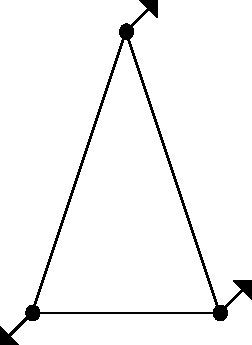
\includegraphics[width=\textwidth]{images/tri_collocated.pdf}
        \caption{Célula triangular co-localizada.}
        \label{fig:tricollo}
    \end{subfigure}
    \hspace{0.1\textwidth}
    \begin{subfigure}[b]{0.23\textwidth}
        \centering
        \includegraphics[width=\textwidth]{images/tri_staggered.pdf}
        \caption{Célula triangular deslocada.}
        \label{fig:tristagg}
    \end{subfigure}
    \subcaption*{Fonte: Elaborada pelo autor.}
    \label{fig:celulas}
\end{figure}

Em geral, simulações de fluidos baseadas em física têm como base as Equações de Navier-Stokes (ENS) para fluidos incompressíveis \cite{incompressible}. Estas são um conjunto de equações diferenciais parciais que descrevem o escoamento dos fluidos. Para resolver as ENS, é necessária a aplicação de operadores diferenciais de cálculo vetorial, tais como: gradiente, divergente e laplaciano. Estes operadores são aplicados em funções contínuas; no entanto, não é possível representar funções contínuas em computadores, logo, estas devem ser discretizadas. Na abordagem euleriana, o método de Diferenças Finitas (do inglês, \textit{Finite Differences} - FD) visa solucionar este problema para grades uniformes. A aplicação de FD em uma célula da grade necessita acessar informações dos vizinhos; estes vizinhos são chamados de estêncil. Em grades uniformes bidimensionais, o estêncil é sempre composto por 4 vizinhos em posições fixas (acima, abaixo, esquerda e direita), conforme mostrado na \figref{fig:stencil2d}. Como esta vizinhança é fixa em grades uniformes, podemos aplicar este método de forma eficiente.

\begin{figure}
    \centering
    \includegraphics[width=0.3\textwidth]{images/stencil-2d.pdf}
    \caption{Estêncil em grade uniforme bidimensional.}
    \subcaption*{Fonte: Elaborada pelo autor.}
    \label{fig:stencil2d}
\end{figure}

Quando trabalhamos com malhas triangulares, temos uma malha não-estruturada. Neste contexto, o conceito de estêncil se torna mais complexo, pois a quantidade e configuração dos vizinhos de uma célula não são mais uniformes. Em malhas não-estruturadas, é comum utilizar o conceito de \textit{k-anel} (do inglês, \textit{k-ring}), que define a vizinhança de um elemento da malha de forma topológica. O \textit{1-anel} de uma célula ou vértice é definido como o conjunto de todos os elementos que compartilham pelo menos uma aresta com o elemento central. Diferentemente do 1-anel em malhas regulares (como mostrado na \figref{fig:stencil2d}), onde sempre há 4 vizinhos em posições fixas, em malhas não-estruturadas o 1-anel pode ter um número variável de vizinhos sem restrições de posição. Por exemplo, em uma malha triangular, o 1-anel de um vértice interno é composto por todos os triângulos que contêm aquele vértice (podendo ser 5, 6, 7 ou mais triângulos), enquanto o 1-anel de um triângulo é formado pelos três triângulos adjacentes que compartilham suas arestas. Este conceito pode ser estendido para \textit{k-anéis}, onde o 2-anel inclui os vizinhos dos vizinhos, e assim sucessivamente. A escolha do tamanho do estêncil (ou seja, quantos anéis incluir) impacta diretamente a precisão e o custo computacional dos métodos numéricos aplicados à malha.

A propriedade de vizinhança variável impossibilita o uso direto de FD em malhas não-estruturadas, sendo necessário o uso de outros métodos para a resolução dos operadores diferenciais, tais como os métodos de Elementos Finitos e Volumes Finitos. Em animação computacional, o método de Volumes Finitos (do inglês, \textit{Finite Volumes} - FV) é o mais utilizado para animação de fluidos em malhas não-estruturadas \cite{Klingner2006}.

Outra propriedade importante de malhas que deve ser considerada é a conformidade. Uma malha conforme (ver \figref{fig:conforme}) é aquela em que todas as arestas são completas, ou seja, não existe um vértice que resida no interior de uma aresta. Na literatura, encontramos diversos trabalhos que lidam com problemas geométricos em malhas não-conformes (ver \figref{fig:africa}) \cite{Mahmood2019, nonconf1}. No entanto, há uma lacuna na resolução das ENS neste tipo de malha. Para resolver numericamente as ENS em malhas não-conformes, é interessante utilizar um método independente da estrutura da malha, isto é, métodos de interpolação sem malha.

\begin{figure}
    \centering
    \caption{Exemplo de malha conforme.}
    \includegraphics[width=0.7\textwidth]{images/africa-conforme.jpg}
    \subcaption*{Fonte: \cite{Nascimento:2014}}
    \label{fig:conforme}
    \vspace{-1.2cm}
\end{figure}

\begin{figure}
    \centering
    \caption{Exemplo de malha não-conforme, com círculo vermelho para evidenciar uma aresta que mostra a propriedade da malha.}
    \includegraphics[width=0.7\textwidth]{images/africa-nao-conforme.png}
    \subcaption*{Fonte: Adaptado de \cite{Nascimento:2014}}
    \label{fig:africa}
\end{figure}

O método baseado em Funções de Base Radial (do inglês, \textit{Radial Basis Function} - RBF) \cite{rbf} realiza uma interpolação independente de malha, e sua aproximação de FD, conhecida como \textit{Radial Basis Function Finite Differences} (RBF-FD) \cite{WRIGHT200699}, resolve os operadores diferenciais necessários. Com a aplicação do RBF-FD em malhas não-conformes, pretendemos resolver as ENS e representar visualmente a simulação de fumaça.

Um desafio fundamental na resolução numérica das ENS é a correta aplicação de condições de fronteira, essenciais para garantir o comportamento físico apropriado do fluido nos limites do domínio. Existem diferentes tipos de condições de fronteira, sendo as mais comuns as condições de Dirichlet, que prescrevem o valor da função no contorno, e as condições de Neumann, que prescrevem o valor da derivada normal no contorno.

Em particular, as condições de Neumann são cruciais para modelar fronteiras com fluxo livre e paredes impermeáveis, mas sua implementação em malhas não-estruturadas apresenta dificuldades significativas. Enquanto métodos tradicionais como FD e FV têm procedimentos bem estabelecidos para aplicar essas condições em grades uniformes, a extensão para malhas triangulares não-conformes utilizando RBF-FD ainda carece de investigação aprofundada na literatura de animação de fluidos.

\section{Objetivos}

O objetivo principal desta dissertação de mestrado é desenvolver uma técnica eficiente de animação de fumaça bidimensional em malhas não-estruturadas utilizando o método RBF-FD, abordando as limitações atuais na aplicação de condições de contorno em malhas triangulares.


\section{Roteiro}

O resto do texto se divide da seguinte maneira. No Capítulo~\ref{chapter:revisao}, abordaremos como evoluiu a simulação de fluidos computacional ao longo do tempo, avaliando os métodos canônicos até os métodos mais atuais. No Capítulo~\ref{chapter:fundteorica}, apresentaremos a fundamentação teórica que baseia nossa solução e enunciaremos os problemas a serem resolvidos. No Capítulo~\ref{chapter:metodologia}, explicaremos os principais métodos utilizados na nossa pesquisa, como o RBF-FD, e como aplicar as condições de contorno de Neumann neste caso. No Capítulo~\ref{chapter:Resultados}, apresentaremos os resultados obtidos com o método proposto, incluindo análise quantitativa do divergente do campo de velocidades e visualização qualitativa das simulações. Por fim, no Capítulo~\ref{chapter:conclusao}, discutiremos as contribuições do trabalho, publicações realizadas e direções para trabalhos futuros.
